\documentclass[12pt,a4paper]{article}

% ─── Page Layout ───────────────────────────────────────────────────────────────
\usepackage[a4paper, margin=0.8in, headheight=14pt]{geometry}

% ─── Fonts (XeLaTeX) ───────────────────────────────────────────────────────────
\usepackage{fontspec}
\usepackage{unicode-math}
\setmainfont{TeX Gyre Pagella}
\setmonofont[Scale=0.88]{TeX Gyre Cursor}
\setmathfont{Latin Modern Math}

% ─── Packages ──────────────────────────────────────────────────────────────────
\usepackage{xcolor}
\usepackage{colortbl}
\usepackage{titlesec}
\usepackage{enumitem}
\usepackage{tabularx}
\usepackage{booktabs}
\usepackage{array}
\usepackage{amsmath}
\usepackage{tikz}
\usetikzlibrary{shapes.geometric, arrows.meta, positioning, calc, fit, decorations.pathreplacing, patterns}
\usepackage[american]{circuitikz}
\usepackage{tcolorbox}
\tcbuselibrary{skins, breakable}
\usepackage{hyperref}
\usepackage{fancyhdr}
\usepackage{graphicx}
\usepackage{microtype}
\hyphenpenalty=10000
\exhyphenpenalty=10000
\sloppy
\usepackage{caption}
\usepackage{setspace}
\usepackage{multirow}
\usepackage{tocloft}

% ─── Q&A helper ────────────────────────────────────────────────────────────────
% Standard macro for Viva Questions
\newcommand{\Q}[1]{\textbf{#1}\par\noindent\ignorespaces}

% ─── Colour Palette ────────────────────────────────────────────────────────────
\definecolor{myred}{RGB}{196,30,58}
\definecolor{mydark}{RGB}{30,30,50}
\definecolor{mygreen}{RGB}{14,120,80}
\definecolor{myteal}{RGB}{0,130,140}
\definecolor{myamber}{RGB}{180,100,0}
\definecolor{mypurple}{RGB}{100,30,160}
\definecolor{mygray}{RGB}{246,247,249}
\definecolor{mgframe}{RGB}{180,185,200}
\definecolor{watermark}{RGB}{145,150,170}
\definecolor{hdrred}{RGB}{250,232,235}
\definecolor{hdrgreen}{RGB}{220,244,233}
\definecolor{hdrteal}{RGB}{220,242,244}
\definecolor{hdramber}{RGB}{253,242,215}
\definecolor{hdrpurple}{RGB}{238,228,255}
\definecolor{hdrgray}{RGB}{238,240,245}
\definecolor{rowalt}{RGB}{250,251,253}

% ─── Section Formatting ────────────────────────────────────────────────────────
\titleformat{\section}{\large\bfseries\color{myred}}{\thesection.}{0.5em}{}[\vspace{1pt}{\color{myred}\rule{\linewidth}{0.8pt}}]
\titleformat{\subsection}{\normalsize\bfseries\color{myteal}}{\thesubsection}{0.5em}{}
\titlespacing*{\section}{0pt}{18pt}{7pt}
\titlespacing*{\subsection}{0pt}{11pt}{4pt}

% ─── Paragraph ─────────────────────────────────────────────────────────────────
\setlength{\parindent}{0pt}
\setlength{\parskip}{4pt}

% ─── TOC Styling ───────────────────────────────────────────────────────────────
\renewcommand{\cfttoctitlefont}{\large\bfseries\color{myred}}
\renewcommand{\cftaftertoctitle}{\par\noindent{\color{myred}\rule{\linewidth}{0.8pt}}}
\setlength{\cftbeforetoctitleskip}{0pt}
\setlength{\cftaftertoctitleskip}{6pt}
\renewcommand{\cftsecfont}{\normalsize\bfseries\color{mydark}}
\renewcommand{\cftsecpagefont}{\normalsize\bfseries\color{mydark}}
\renewcommand{\cftsecleader}{\cftdotfill{\cftdotsep}}
\setlength{\cftbeforesecskip}{7pt}
\renewcommand{\cftsubsecfont}{\small\color{mydark}}
\renewcommand{\cftsubsecpagefont}{\small\color{mydark}}
\setlength{\cftbeforesubsecskip}{3pt}
\setlength{\cftsubsecindent}{1.4em}

% ─── Table helpers ─────────────────────────────────────────────────────────────
\renewcommand{\arraystretch}{1.45}
\setlength{\tabcolsep}{6pt}
\arrayrulecolor{mydark}
\newcolumntype{B}[1]{>{\small\bfseries\raggedright\arraybackslash}m{#1}}
\newcolumntype{Y}{>{\small\raggedright\arraybackslash}X}
\renewcommand{\tabularxcolumn}[1]{m{#1}}

% ─── Header / Footer ───────────────────────────────────────────────────────────
\pagestyle{fancy}
\fancyhf{}
\fancyhead[L]{\small\color{myred}\textbf{PE-EC802A}\;\color{mydark}--- Mixed Signal Design}
\fancyhead[R]{\small\color{myteal}\textbf{Module 2 Notes}}
\fancyfoot[C]{\small\color{mydark}\thepage}
\fancyfoot[R]{\small\color{watermark}\textit{\copyright\ Biraj}}
\renewcommand{\headrulewidth}{0.5pt}
\renewcommand{\footrulewidth}{0.3pt}

% ─── Hyperref ──────────────────────────────────────────────────────────────────
\hypersetup{colorlinks=true, linkcolor=myteal, urlcolor=myteal,
  pdfauthor={Biraj Sarkar}, pdftitle={PE-EC802A --- Module 2 Notes}}

% ─── tcolorbox styles ──────────────────────────────────────────────────────────
\tcbset{
  tikzbox/.style={colback=mygray, colframe=mgframe, boxrule=0.6pt, arc=4pt,
    left=8pt, right=8pt, top=6pt, bottom=6pt,
    colbacktitle=mgframe, coltitle=mydark, fonttitle=\small\bfseries},
  defbox/.style={colback=hdrgreen, colframe=mygreen, boxrule=0.8pt, arc=4pt,
    left=9pt, right=9pt, top=6pt, bottom=6pt,
    colbacktitle=mygreen, coltitle=white, fonttitle=\small\bfseries},
  formulabox/.style={colback=hdrteal, colframe=myteal, boxrule=0.8pt, arc=4pt,
    left=9pt, right=9pt, top=7pt, bottom=7pt,
    colbacktitle=myteal, coltitle=white, fonttitle=\small\bfseries},
  examplebox/.style={colback=hdramber, colframe=myamber, boxrule=0.8pt, arc=4pt,
    left=9pt, right=9pt, top=6pt, bottom=6pt,
    colbacktitle=myamber, coltitle=white, fonttitle=\small\bfseries},
  masonbox/.style={colback=hdrpurple, colframe=mypurple, boxrule=0.8pt, arc=4pt,
    left=9pt, right=9pt, top=6pt, bottom=6pt,
    colbacktitle=mypurple, coltitle=white, fonttitle=\small\bfseries},
  exambox/.style={colback=hdrpurple, colframe=mypurple, boxrule=1pt, arc=5pt,
    left=10pt, right=10pt, top=8pt, bottom=8pt,
    colbacktitle=mypurple, coltitle=white, fonttitle=\bfseries,
    breakable, title after break={\textbf{Frequently Asked / Viva Questions (contd.)}}}
}
\tcbset{breakable}

% ─── TikZ styles ───────────────────────────────────────────────────────────────
\tikzset{
  block/.style={rectangle, draw=myteal, fill=hdrteal,
    text width=2.4cm, align=center, minimum height=0.95cm,
    font=\small, rounded corners=3pt, line width=0.7pt},
  redblock/.style={rectangle, draw=myred, fill=hdrred,
    text width=2.4cm, align=center, minimum height=0.95cm,
    font=\small, rounded corners=3pt, line width=0.7pt},
  sumjunc/.style={circle, draw=myamber, fill=hdramber,
    minimum size=0.62cm, font=\small, line width=0.8pt},
  arrow/.style={-Stealth, thick, color=mydark},
  line/.style={thick, color=mydark}
}

% ═══════════════════════════════════════════════════════════════════════════════
\begin{document}
% ═══════════════════════════════════════════════════════════════════════════════

\begin{center}
  {\LARGE\bfseries\color{myred} PE-EC802A --- Mixed Signal Design}\\[5pt]
  {\normalsize\color{mydark} Semester VIII \quad$\bullet$\quad 3L:0T:0P \quad$\bullet$\quad 3 Credits}\\[3pt]
  {\normalsize\color{myteal}\textbf{Module 2 Exam Notes}}\\[3pt]
  {\small\color{mydark} CGEC \;$|$\; B.Tech ECE (2023--27) \;$|$\; \textit{Biraj Sarkar}}
\end{center}
\vspace{2pt}
\noindent{\color{myred}\rule{\linewidth}{1.5pt}}
\vspace{2pt}

\hypersetup{linkcolor=mydark}
\tableofcontents
\hypersetup{linkcolor=myteal}
\newpage

% ===============================================================================
\section{Switched-Capacitor (SC) Circuits \& Resistor Equivalence}
% ===============================================================================

\begin{tcolorbox}[defbox, title={\textbf{Switched-Capacitor Circuit Concept}}]
A \textbf{Switched-Capacitor (SC) circuit} is a discrete-time signal processing circuit that implements resistors by rapidly switching charge back and forth between capacitors using non-overlapping clock phases. SC circuits are highly preferred in CMOS technology because precise on-chip resistors are difficult to fabricate, whereas capacitor ratios can be matched with extremely high accuracy (up to $0.1\%$).
\end{tcolorbox}

\subsection{Switched-Capacitor Filter Architectures}
A practical SC biquad (second-order section) is built using two SC integrators in a feedback loop. The \textbf{Fleischer-Laker biquad} is the standard SC biquad implementing LP, HP, and BP outputs simultaneously.

\begin{tcolorbox}[tikzbox, title={Fleischer-Laker SC Biquad Block Structure}]
\centering
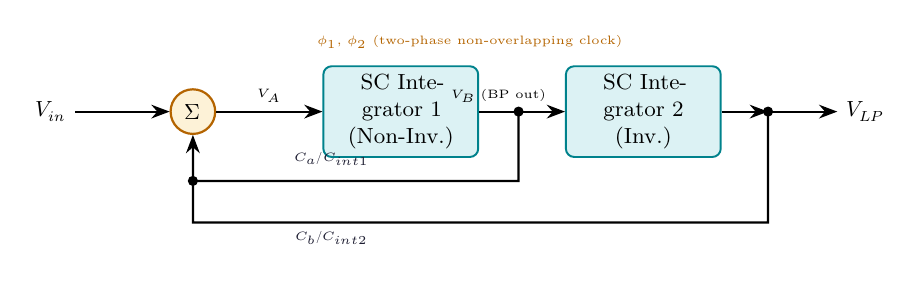
\begin{tikzpicture}[scale=0.88, transform shape]
  % Two SC integrator blocks
  \node[block, text width=2.0cm] (int1) at (1.5, 0) {SC Integrator 1\\ (Non-Inv.)};
  \node[block, text width=2.0cm] (int2) at (5.0, 0) {SC Integrator 2\\ (Inv.)};
  \node[sumjunc] (sum) at (-1.5, 0) {$\Sigma$};

  % Forward path
  \draw[-Stealth, thick] (sum.east) -- (int1.west) node[midway, above, font=\tiny]{$V_A$};
  \draw[thick] (int1.east) -- (3.2, 0) node[midway, above, font=\tiny]{$V_B$ (BP out)};
  \draw[-Stealth, thick] (3.2, 0) -- (int2.west);
  \draw[-Stealth, thick] (int2.east) -- (6.8, 0);
  \draw[-Stealth, thick] (6.8, 0) -- (7.8, 0) node[right, font=\small]{$V_{LP}$};

  % Feedback paths
  \draw[thick] (6.8, 0) to[short, *-] (6.8, -1.6) -- (-1.5, -1.6) -- (-1.5, -1.0);
  \draw[thick] (3.2, 0) to[short, *-] (3.2, -1.0) to[short, -*] (-1.5, -1.0);
  \draw[-Stealth, thick] (-1.5, -1.0) -- (sum.south);

  % Input
  \draw[-Stealth, thick] (-3.2, 0) node[left, font=\small]{$V_{in}$} -- (sum.west);

  % Capacitor ratio labels on feedback
  \node[above, font=\tiny\color{mydark}] at (0.5, -0.9) {$C_a/C_{int1}$};
  \node[below, font=\tiny\color{mydark}] at (0.5, -1.6) {$C_b/C_{int2}$};

  % Clock label
  \node[font=\tiny, color=myamber] at (2.5, 1.0) {$\phi_1$, $\phi_2$ (two-phase non-overlapping clock)};
\end{tikzpicture}
\end{tcolorbox}

\textbf{How the Fleischer-Laker Biquad Sets Frequency and Q:}
\begin{itemize}[leftmargin=*, itemsep=2pt]
  \item Pole frequency: $\omega_0 \propto \frac{f_{clk} \cdot C_{sampling}}{C_{integrating}}$ --- set purely by capacitor ratios and clock frequency.
  \item Quality factor $Q$: set by the feedback capacitor ratio. Changing $C_a$ and $C_b$ independently controls $\omega_0$ and $Q$ without interaction.
\end{itemize}

\subsection{Switched-Capacitor Filter Applications}
\begin{itemize}[leftmargin=*, itemsep=2.5pt]
  \item \textbf{Audio CODEC:} Anti-aliasing and reconstruction filters in 16--24-bit audio codecs (e.g., CD player, smartphone DAC) where precise $\pm 0.01\%$ corner frequency tolerance is required.
  \item \textbf{$\Delta\Sigma$ ADC Front-End:} SC integrators inside $\Delta\Sigma$ modulators perform the summation and integration operations that shape quantization noise to high frequencies.
  \item \textbf{DTMF (Dual-Tone Multi-Frequency) Decoding:} Narrow-band bandpass SC filters detect individual telephone dial tones.
  \item \textbf{Biomedical Instrumentation:} Low-frequency, high-accuracy SC filters for ECG/EEG signal conditioning, where process-insensitive frequency accuracy is essential.
\end{itemize}

\subsection{Derivation of SC Resistor Equivalence}
Consider a capacitor $C$ connected between two voltage nodes $V_1$ and $V_2$ via two single-pole single-throw switches controlled by non-overlapping clock phases $\Phi_1$ and $\Phi_2$ with a clock frequency $f_c = 1/T_c$.

\begin{tcolorbox}[tikzbox, title={Switched-Capacitor Resistor Equivalence Circuit}]
\centering
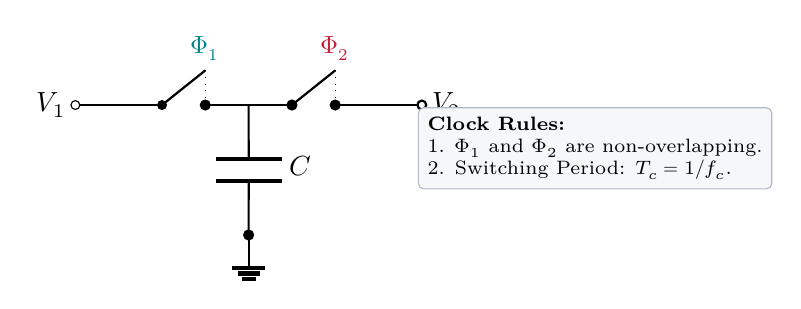
\begin{tikzpicture}[scale=1.1]
  % Nodes
  \draw (0,0) node[left] {$V_1$} to[short, o-*] (1,0);
  
  % Switch 1 (Phi 1)
  \draw[thick] (1,0) -- (1.5,0.4) node[above, font=\small\color{myteal}] {$\Phi_1$};
  \draw[dotted] (1.5,0.4) -- (1.5,0);
  \draw[thick] (1.5,0) to[short, *-*] (2.5,0);
  
  % Switch 2 (Phi 2)
  \draw[thick] (2.5,0) -- (3.0,0.4) node[above, font=\small\color{myred}] {$\Phi_2$};
  \draw[dotted] (3.0,0.4) -- (3.0,0);
  \draw[thick] (3.0,0) to[short, *-o] (4.0,0) node[right] {$V_2$};
  
  % Capacitor
  \draw[thick] (2.0,0) to[C, l=$C$, -*] (2.0,-1.5) node[ground] {};
  
  % Timing diagram / Clock phase labeling
  \node[draw=mgframe, fill=mygray, rounded corners=2pt, font=\scriptsize, align=left] at (6.0,-0.5) {
    \textbf{Clock Rules:}\\
    1. $\Phi_1$ and $\Phi_2$ are non-overlapping.\\
    2. Switching Period: $T_c = 1/f_c$.
  };
\end{tikzpicture}
\end{tcolorbox}

\textbf{Step-by-step Derivation:}
\begin{enumerate}[label=\textbf{\arabic*.}, leftmargin=*, itemsep=3pt]
  \item During phase $\Phi_1$, Switch 1 is closed and Switch 2 is open. The capacitor $C$ charges to voltage $V_1$.
  The charge stored on the capacitor is:
  \[
  Q_1 = C V_1
  \]
  \item During phase $\Phi_2$, Switch 1 opens and Switch 2 closes. The capacitor $C$ is connected to $V_2$, charging or discharging to $V_2$.
  The charge remaining on the capacitor is:
  \[
  Q_2 = C V_2
  \]
  \item The net charge transferred from node $V_1$ to node $V_2$ in one clock period $T_c$ is:
  \[
  \Delta Q = Q_1 - Q_2 = C(V_1 - V_2)
  \]
  \item The average current $I_{avg}$ flowing from node $V_1$ to node $V_2$ is the charge transferred per unit time:
  \[
  I_{avg} = \frac{\Delta Q}{T_c} = \frac{C(V_1 - V_2)}{T_c} = f_c C (V_1 - V_2)
  \]
  \item Using Ohm's Law ($I = \frac{V_1 - V_2}{R_{eq}}$), we find the equivalent resistance $R_{eq}$ of the switched-capacitor stage:
  \begin{tcolorbox}[formulabox, title={\textbf{SC Equivalent Resistance}}]
  \[
  R_{eq} = \frac{V_1 - V_2}{I_{avg}} = \frac{1}{f_c C}
  \]
  where:
  \begin{itemize}[leftmargin=1.5em, itemsep=1pt]
    \item $R_{eq} = $ Equivalent resistance ($\Omega$)
    \item $f_c = $ Clock switching frequency (Hz)
    \item $C = $ Capacitance (F)
  \end{itemize}
  \end{tcolorbox}
\end{enumerate}

\subsection{Significance of SC Circuits in IC Design}
In integrated circuits, fabricating large resistors (e.g., $100\,$k$\Omega$) is highly impractical because:
\begin{itemize}[leftmargin=*, itemsep=2pt]
  \item \textbf{Area:} Polysilicon/diffusion resistors require massive silicon area.
  \item \textbf{Accuracy:} Absolute tolerances of resistors on silicon are poor ($\pm 20\%$) and drift significantly with temperature.
  \item \textbf{Tuning:} RC time constants ($\tau = RC$) vary by up to $40\%$ due to process variations.
\end{itemize}
In contrast, in SC circuits, the equivalent time constant of an integrator is:
\[
\tau = R_{eq} C_2 = \left(\frac{1}{f_c C_1}\right) C_2 = \frac{1}{f_c} \left(\frac{C_2}{C_1}\right)
\]
Since $f_c$ is derived from a highly stable crystal oscillator and $\frac{C_2}{C_1}$ is a ratio of two matched capacitors (which matches perfectly within $0.1\%$ on layout), the time constant $\tau$ is extremely accurate and temperature-independent.

% ===============================================================================
\section{SC Non-Idealities \& Mitigation Strategies}
% ===============================================================================

In real CMOS processes, MOS transistors act as non-ideal switches. The key non-idealities are:

\subsection{1. Charge Injection}
When a MOS switch is turned ON, a channel charge $Q_{ch}$ is accumulated in the inversion layer:
\[
Q_{ch} = W L C_{ox} (V_{GS} - V_{TH}) = W L C_{ox} (V_{CLK} - V_{in} - V_{TH})
\]
When the switch is turned OFF (gate voltage drops), this channel charge is released and flows out through the source and drain terminals. The charge injected into the sampling capacitor $C$ shifts the sampled voltage, introducing an offset and non-linear distortion (since $V_{TH}$ depends non-linearly on $V_{in}$ via the body effect).

\subsection{2. Clock Feedthrough}
The overlap capacitance $C_{ov}$ between the gate and source/drain terminals forms a capacitive voltage divider with the sampling capacitor. The clock transition at the gate is directly coupled to the sampling capacitor:
\[
\Delta V = V_{CLK} \left( \frac{C_{ov}}{C_{ov} + C} \right)
\]
This introduces a constant offset voltage to the sampled signal.

\subsection{3. thermal Noise ($k_B T / C$ Noise)}
An ON transistor has a finite channel resistance $R_{on}$. This resistance generates thermal noise with a power spectral density of $4 k_B T R_{on}$. When the switch is opened, this noise is sampled onto the capacitor. The total noise power integrated over the loop bandwidth is:
\begin{tcolorbox}[formulabox, title={\textbf{Thermal Noise Limit (kT/C)}}]
\[
v_n^2 = \int_0^{\infty} \frac{4 k_B T R_{on}}{1 + (2\pi f R_{on} C)^2} df = \frac{k_B T}{C}
\]
where $k_B$ is the Boltzmann constant ($1.38 \times 10^{-23}$ J/K) and $T$ is temperature in Kelvin.
\end{tcolorbox}
This noise sets a fundamental limit on the dynamic range (SNDR) of switched-capacitor circuits. To achieve higher resolution, $C$ must be made larger, which increases power consumption and area.

\begin{tcolorbox}[tikzbox, title={Summary of Switch Mitigation Techniques}]
\centering
\par\noindent
\begin{tabularx}{\linewidth}{|B{3.5cm}|Y|Y|}
\hline
\textbf{Non-Ideality} & \textbf{Physical Mechanism} & \textbf{Mitigation Strategy} \\ \hline
\textbf{Charge Injection} & Channel charge flows into $C$ upon turn-off & Dummy switches, differential signaling, bottom-plate sampling \\ \hline
\textbf{Clock Feedthrough} & Overlap capacitance $C_{ov}$ couples clock edges & CMOS transmission gates, differential architectures \\ \hline
\textbf{Thermal Noise} & Thermal noise of $R_{on}$ is sampled onto $C$ & Increase capacitance value $C$ ($v_n \propto 1/\sqrt{C}$) \\ \hline
\end{tabularx}
\end{tcolorbox}

% ===============================================================================
\section{Stray-Insensitive Integrators}
% ===============================================================================

Early SC designs were sensitive to parasitic capacitances between node terminals and substrate (ground), causing gain errors. Modern SC systems use \textbf{stray-insensitive} configurations.

\subsection{Stray-Insensitive Non-Inverting Integrator}
The stray-insensitive non-inverting integrator uses 4 switches controlled by non-overlapping clocks $\Phi_1$ and $\Phi_2$.

\begin{tcolorbox}[tikzbox, title={Stray-Insensitive Non-Inverting SC Integrator Circuit}]
\centering
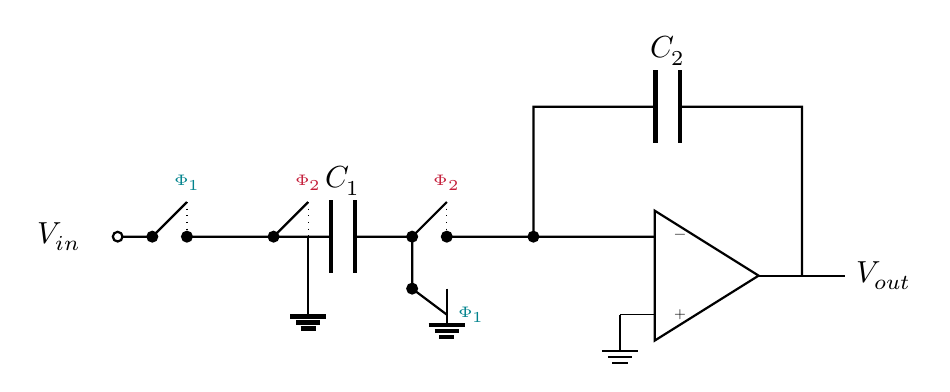
\begin{tikzpicture}[scale=1.1, transform shape]
  % Op-amp
  \draw[thick] (5, 0) -- (5, -1.5) -- (6.2, -0.75) -- cycle;
  \node[font=\tiny] at (5.3, -0.3) {$-$};
  \node[font=\tiny] at (5.3, -1.2) {$+$};
  \draw (5, -1.2) -- (4.6, -1.2) node[ground] {};
  \draw[thick] (6.2, -0.75) -- (7.2, -0.75) node[right] {$V_{out}$};

  % Input node and switches
  \node[left] at (-1.5, -0.3) {$V_{in}$};
  \draw[thick] (-1.2, -0.3) to[short, o-*] (-0.8, -0.3);
  
  % Switch S1 (Phi 1)
  \draw[thick] (-0.8, -0.3) -- (-0.4, 0.1) node[above, font=\tiny\color{myteal}] {$\Phi_1$};
  \draw[dotted] (-0.4, 0.1) -- (-0.4, -0.3);
  \draw[thick] (-0.4, -0.3) to[short, *-*] (0.6, -0.3);

  % Switch S2 (Phi 2)
  \draw[thick] (0.6, -0.3) -- (1.0, 0.1) node[above, font=\tiny\color{myred}] {$\Phi_2$};
  \draw[dotted] (1.0, 0.1) -- (1.0, -0.3);
  \draw[thick] (1.0, -0.3) -- (1.0, -0.8) node[ground] {};

  % Input Capacitor C1
  \draw[thick] (0.6, -0.3) to[C, l=$C_1$, -*] (2.2, -0.3);

  % Switch S3 (Phi 2)
  \draw[thick] (2.2, -0.3) -- (2.6, 0.1) node[above, font=\tiny\color{myred}] {$\Phi_2$};
  \draw[dotted] (2.6, 0.1) -- (2.6, -0.3);
  \draw[thick] (2.6, -0.3) to[short, *-*] (3.6, -0.3) -- (5, -0.3);

  % Switch S4 (Phi 1)
  \draw[thick] (2.2, -0.3) -- (2.2, -0.8) to[short, -*] (2.2, -0.9);
  \draw[thick] (2.2, -0.9) -- (2.6, -1.2) node[right, font=\tiny\color{myteal}] {$\Phi_1$};
  \draw[dotted] (2.6, -1.2) -- (2.6, -0.9);
  \draw[thick] (2.6, -0.9) node[ground] {};

  % Feedback Capacitor C2
  \draw[thick] (3.6, -0.3) -- (3.6, 1.2) to[C, l=$C_2$] (6.7, 1.2) -- (6.7, -0.75);
  \draw[thick] (6.7, -0.75) -- (6.2, -0.75);
\end{tikzpicture}
\end{tcolorbox}

\textbf{Analysis of Stray Insensitivity:}
\begin{itemize}[leftmargin=*, itemsep=2.5pt]
  \item \textbf{Node A (left plate of $C_1$):} Connected to either $V_{in}$ (low impedance source) during $\Phi_1$ or to ground during $\Phi_2$. Any parasitic capacitor at this node is either charged by $V_{in}$ or fully discharged to ground, never affecting the charge transferred to the integrating capacitor $C_2$.
  \item \textbf{Node B (right plate of $C_1$):} Connected to virtual ground (op-amp inverting terminal) during $\Phi_2$ or to physical ground during $\Phi_1$. The potential is always at ground (virtual or physical), so the voltage across its parasitics is always $0\,$V. Thus, no charge is stored or injected by the parasitic capacitance.
\end{itemize}

\subsection{Charge Equations and Transfer Function}
Let us write the discrete-time charge conservation equation at the virtual ground node:
\begin{enumerate}[label=\textbf{\arabic*.}, leftmargin=*, itemsep=3pt]
  \item During $\Phi_1(n-1)$, $C_1$ charges to $V_{in}(n-1)$ (left terminal to $V_{in}$, right terminal to ground).
  \[
  q_{C1}(n-1) = C_1 V_{in}(n-1)
  \]
  \item During $\Phi_2(n)$, $C_1$ is connected to ground on the left and virtual ground on the right. The capacitor is fully discharged, and its charge flows entirely into $C_2$. The feedback capacitor $C_2$ accumulates this charge:
  \[
  C_2 V_{out}(n) = C_2 V_{out}(n-1) + C_1 V_{in}(n-1)
  \]
  \item Taking the Z-transform of this difference equation:
  \[
  C_2 Y(z) = C_2 z^{-1} Y(z) + C_1 z^{-1} X(z)
  \]
  \[
  Y(z)(1 - z^{-1}) = \frac{C_1}{C_2} z^{-1} X(z)
  \]
  \item The transfer function $H(z) = Y(z)/X(z)$ is:
  \begin{tcolorbox}[formulabox, title={\textbf{Non-Inverting SC Integrator Transfer Function}}]
  \[
  H(z) = \frac{V_{out}(z)}{V_{in}(z)} = \frac{C_1}{C_2} \frac{z^{-1}}{1 - z^{-1}}
  \]
  \end{tcolorbox}
  The term $z^{-1}$ in the numerator indicates a delay of one clock cycle, making this a \textbf{delaying (non-inverting) integrator}.
\end{enumerate}

If we modify the switch network such that $C_1$ is connected to $V_{in}$ and virtual ground during the same clock phase, we obtain an \textbf{inverting (non-delaying) integrator} with transfer function:
\[
H(z) = -\frac{C_1}{C_2} \frac{1}{1 - z^{-1}}
\]

% ===============================================================================
\section{First-Order \& Second-Order SC Filters (Biquads)}
% ===============================================================================

\subsection{Fleischer-Laker Biquad Topology}
The Fleischer-Laker biquad is a standard stray-insensitive second-order SC filter stage. It consists of two op-amps and a network of switched and unswitched capacitors. It can implement low-pass, high-pass, band-pass, and notch transfer functions by selecting appropriate capacitor ratios.

The general Z-domain transfer function of a second-order SC biquad is given by:
\[
H(z) = \frac{N(z)}{D(z)} = \frac{\alpha_0 + \alpha_1 z^{-1} + \alpha_2 z^{-2}}{1 + \beta_1 z^{-1} + \beta_2 z^{-2}}
\]
By mapping s-plane specifications (e.g. pole frequency $\omega_0$ and quality factor $Q$) through the Bilinear Transformation, the discrete coefficients $\alpha_i$ and $\beta_i$ are determined, allowing direct calculation of the required capacitor ratios.

% ===============================================================================
% QUICK REVISION PAGE
% ===============================================================================
\newpage
\begin{center}
  {\large\bfseries\color{myred} Quick Revision --- Module 2}\\[3pt]
  {\small\color{mydark} Switched-Capacitor Filters $|$ PE-EC802A}
\end{center}
\noindent{\color{myred}\rule{\linewidth}{1.2pt}}
\vspace{4pt}

\begin{tcolorbox}[formulabox, title={\textbf{Key Formulas at a Glance}}]
\renewcommand{\arraystretch}{1.35}
\begin{tabularx}{\linewidth}{B{5.0cm} X}
Equivalent Resistance & $R_{eq} = \frac{1}{f_c C}$ \\[4pt]
Integrator Time Constant & $\tau = \frac{1}{f_c} \left( \frac{C_2}{C_1} \right)$ \\[4pt]
Thermal Noise Power & $v_n^2 = \frac{k_B T}{C}$ \\[4pt]
Non-Inverting SC Integrator & $H(z) = \frac{C_1}{C_2} \frac{z^{-1}}{1 - z^{-1}}$ \\[4pt]
Inverting SC Integrator & $H(z) = -\frac{C_1}{C_2} \frac{1}{1 - z^{-1}}$ \\[4pt]
Channel Charge & $Q_{ch} = W L C_{ox}(V_{CLK} - V_{in} - V_{TH})$ \\[4pt]
Clock Feedthrough Offset & $\Delta V = V_{CLK} \left( \frac{C_{ov}}{C_{ov} + C} \right)$ \\
\end{tabularx}
\end{tcolorbox}

\begin{tcolorbox}[defbox, title={\textbf{One-Line Definitions}}]
\begin{itemize}[leftmargin=*, itemsep=2pt, topsep=0pt]
  \item \textbf{SC Resistor Equivalence:} A capacitor switched at high rate acts as a resistor of value $1/(f_c C)$.
  \item \textbf{Non-overlapping Clocks:} Clock signals $\Phi_1$ and $\Phi_2$ that are never high at the same time to prevent direct shorting.
  \item \textbf{Charge Injection:} Channel charge of a switching MOS transistor entering the sampling capacitor upon turn-off.
  \item \textbf{Clock Feedthrough:} Direct capacitive coupling of the clock transition to the node via overlap capacitance.
  \item \textbf{Stray-Insensitive Integrator:} SC integrator topology immune to parasitics of capacitors to substrate/ground.
  \item \textbf{kT/C Noise:} The fundamental thermodynamic limit on sampled voltage accuracy, equal to $k_B T / C$.
  \item \textbf{Stray-Insensitive SC Integrator:} An SC integrator topology where parasitic capacitances at the virtual ground node of the op-amp are shielded and do not contribute to the transfer function.
\end{itemize}
\end{tcolorbox}

\begin{tcolorbox}[tikzbox, title={\textbf{Continuous-Time vs.~Switched-Capacitor Filter Comparison}}]
\centering
\par\noindent
\renewcommand{\arraystretch}{1.3}
\begin{tabularx}{\linewidth}{|B{2.8cm}|Y|Y|}
\hline
\textbf{Property} & \textbf{Active RC Filter} & \textbf{Switched-Capacitor Filter} \\ \hline
\textbf{$\omega_c$ accuracy} & Depends on absolute $R$, $C$ ($\pm20\%$) & Set by $C$ ratio $\times$ $f_{clk}$ ($<0.1\%$) \\ \hline
\textbf{Tuning} & Manual trim required & Reprogram $f_{clk}$ \\ \hline
\textbf{Frequency range} & DC to $>1\,$GHz & DC to $\sim f_{clk}/2$ (audio/kHz range) \\ \hline
\textbf{Clock noise} & Not applicable & Clock feedthrough adds noise floor \\ \hline
\textbf{Silicon area} & Needs large R, C & Compact (capacitors only) \\ \hline
\textbf{CMOS compatible} & Requires resistors & Fully CMOS-compatible \\ \hline
\end{tabularx}
\end{tcolorbox}

\begin{tcolorbox}[exambox, title={\textbf{Frequently Asked / Viva Questions}}]
\begin{enumerate}[topsep=0pt, label=\textbf{Q\arabic*.}, itemsep=5pt]
  \item \Q{Derive the equivalent resistance of a switched capacitor.}
    A capacitor $C$ charged to $V_1$ at phase $\Phi_1$ holds charge $Q_1 = C V_1$. At phase $\Phi_2$, it discharges to $V_2$, holding charge $Q_2 = C V_2$. The net charge transferred per cycle is $\Delta Q = C(V_1-V_2)$. The average current is $I_{avg} = \Delta Q / T_c = f_c C (V_1-V_2)$. Since $R_{eq} = (V_1-V_2)/I_{avg}$, we get $R_{eq} = 1/(f_c C)$.
  \item \Q{Why are switched-capacitor circuits preferred over continuous-time active RC circuits on-chip?}
    Precise resistors are hard to fabricate in CMOS (requiring huge area and having $\pm 20\%$ variations). SC circuits replace resistors with capacitors. The time constant depends on the ratio of two matched capacitors, which matches within $0.1\%$, providing highly precise and temperature-stable performance.
  \item \Q{What is kT/C noise and what limits does it impose?}
    It is the thermal noise power sampled onto a capacitor from the switch channel resistance. It is independent of the switch resistance and equals $k_B T / C$. It sets a lower limit on signal resolution; higher dynamic range requires larger capacitors.
  \item \Q{Explain the mechanism of charge injection in MOS switches.}
    When an MOS transistor is ON, it has charge in its inversion channel. When it turns OFF, this charge exits through the source and drain terminals, injecting charge into the sampling capacitor, shifting the voltage and causing non-linear distortion.
  \item \Q{How does a dummy switch mitigate charge injection?}
    A dummy transistor (usually half the size of the main switch with source/drain shorted) is connected in series. It is driven by the complementary clock. When the main switch turns OFF and releases charge, the dummy switch turns ON and absorbs that charge, neutralizing the error.
  \item \Q{What is bottom-plate sampling, and why is it stray-insensitive?}
    It is a switching technique where the switch connected to the virtual ground (bottom plate) is opened slightly before the input switch. Since the bottom plate is at virtual ground, the charge injected is constant and independent of the input voltage, eliminating non-linear distortion.
  \item \Q{Show the Z-domain transfer function of a non-inverting SC integrator.}
    It is $H(z) = \frac{C_1}{C_2} \frac{z^{-1}}{1 - z^{-1}}$, which represents a delaying integrator.
  \item \Q{Compare inverting and non-inverting SC integrator transfer functions.}
    The inverting integrator is non-delaying: $H(z) = -\frac{C_1}{C_2} \frac{1}{1-z^{-1}}$. The non-inverting integrator has a delay: $H(z) = \frac{C_1}{C_2} \frac{z^{-1}}{1-z^{-1}}$.
  \item \Q{What is the Fleischer-Laker biquad?}
    It is a stray-insensitive, second-order switched-capacitor filter topology capable of implementing any generic second-order transfer function (LP, HP, BP, Notch) by choosing appropriate capacitor values.
  \item \Q{What is clock feedthrough and how is it reduced?}
    Clock feedthrough is the coupling of the clock gate signal to the sampling capacitor via the MOS gate-overlap capacitances. It is reduced by using transmission gates (where PMOS and NMOS cancel each other's transitions) or differential architectures.
\end{enumerate}
\end{tcolorbox}

\end{document}
